%Literature Survey

\section{Overview of Partial Discharge}

\subsection{Partial discharge phenomenon}
Partial discharges are a symptom of deterioration of insulation of the current transformer winding. Thus, partial discharge testing helps in determining the maintenance requirements of such high voltage Current Transformers\setlength{\parskip}{1em}.

Partial Discharge testing can be done On line or Off line which indicates that partial discharges indeed do occur. The partial discharges may only occur for a short time before failure with some types of failure mechanisms To prevent in-service failures of Current Transformers, continuous monitoring is necessary. Inexpensive continuous partial discharge monitor is available. The partial discharge monitoring will only be cost-effective for very critical process for high voltage current Transformers where in-service failures may have large financial consequence

The confirmation of the occurrence of partial discharges depends on the experience of the maintenance staff. The partial discharges characteristics caused by failures can ~be ~distinguished ~by ~noises ~and ~evaluating ~the time, ~voltage ~and ~phase characteristics. The phase is useful in investigating characteristics \cite{kim2003acoustic}.

Research activities are carried out on partial discharges phenomenon in solid, liquid and gaseous insulating materials used in high voltage current Transformers. The input voltage to the Current Transformers plays a significant role on the partial discharges. Phase shift during discharge occurrence can relate with the role of the space charge around the discharge sites in solid and liquid materials. The effects of partial discharges in solid are different with partial discharges in the liquid material. The Partial discharge magnitude in solid as well as in liquid strongly depends on partially applied voltage. Partial discharge probability in solid is strongly dependent on the time derivative of the applied voltage, but discharge probability in the liquid is strongly affected by the instantaneous applied voltage \cite{chen2008partial, forssen2008partial, standard200060270}. 

Partial Discharge generates the signals which can be detected by acoustic sensors. Partial discharge sources in current transformers can be detected by using acoustic methods. For the acoustic method, the signals of constant velocity are detected by acoustic a sensor which gives feedback on insulation condition of the solid and liquid material. Sometimes when the velocities of signals are not constant and will detect the wrong location of partial discharge. The pulses generated by partial discharge phenomenon may deform before reaching to the sensors and will give wrong indications. The deformation of the pulse depends upon the medium of pulse and distance traveled by the pulse. Thus sensor signaling cannot be correct representation partial discharge. Thus incorrect signals will give wrong sensing and fault detection of partial discharge. The location of the source of partial discharge can be known from the frequency of input pulse detection by the sensor which helps in identifying location of partial discharge inside the instrument.

 The Partial discharge detection system in high voltage equipment contains an analysis of distribution. The discharge on the surface or internal insulation failure causes the weakening strength of insulation over the period and lead to total failure of insulation system to avoid the effect on the life of insulation it is necessary to measure the discharge and internal condition of an instrument \cite{kuffel2000high2}.
 
Now a day's transmission line voltage level has increased above 400 kV line to 765 kV, 1000 kV, 1200 kV due to rise in demand of electrical energy. The advantage of high voltage line, transmission line loss is reduced but requires very high level of insulation. 

When the field intensity level goes above a particular level in high voltage equipment, generation of nonuniform field causes weakening of solid, liquid or gaseous insulation. The discharge direction depends upon the energy level generated by the partial discharge phenomenon. The partial discharge analysis depends upon the magnitude of discharge, insulation weakening and voltage level \cite{gockenbach2004partial}

In our study, a high voltage current transformer 145 kV up to 3000 A is selected. A detailed description including technical details of the test set up, graphical analysis of PD distributions of the sample with observation table and conclusions obtained are mentioned.

The partial discharge analysis in solid insulation can be done by the electro-optical measurement system.

Partial discharge monitoring can be done Online to avoid failure of power equipment. Acoustic emission is suitable to measure online partial discharge. The effect of partial discharge on insulation depends upon the magnitude and strength of Partial discharges. The deterioration of insulation is different for partial discharge pulses. The acoustic emissions are detected by the sensors inside the instrument. The signals issued by sensors are given to oscilloscope connected to the computer. The amplitude of the signal is analyzed for frequency magnitude, median, band, and these parameters are used for knowing the level of partial discharges \cite{bengtsson1996status}.

The high voltage equipment is under electrical stress which discharges energy due to the internal dissipation of energy from the various insulating material, hence consideration is given during design to decide insulating parameters, material, the distance between live parts. The electronic equipment which operates at high switching frequencies produces a corona. The corona voltages at high frequency are lower than the breakdown voltage. The breakdown data can be obtained from 10 kHz to 30 kHz frequency \cite{naiduhigh2}.

In liquid insulation oil, the partial discharge looks as streamers. Due to electric stress in equipment, this discharge in the insulation affects the performance of insulation. The partial discharge in oil is always due to the nonuniform field.

 The partial discharges are defined as a charge in Coulomb q. Generally, the value of partial discharge is E-9 hence defined in pC and phase angle in degree. The partial discharge phenomenon takes place in both cycles of a sine wave. As per the literature available, partial discharge pulses are higher, but the magnitude is small in the negative half cycle. The partial discharge pulse reaches to the peak value when the voltage reaches the peak. Thus it proves that PD pulse depends strongly upon the value of applied voltage. The streamer discharge in oil insulating material is used through oscilloscope for simulation using the electrical circuit. The pattern of simulated PD is compared with the discharge results obtained by calculation or experiment \cite{kim2003acoustic, nattrass1993partial, macalpine2002development, kemp1995partial}.
 
The Partial discharge can be measured by analysis method, acoustic or electro technological diagnostics. This test performs insulation strength of electrical devices in the system. There are many methods detecting partial discharge in high voltage equipment. The laboratory testing methods are available for solid and liquid insulating samples. In experiments, flat samples are generated with exposure to field conditions and partial discharge are simulated for measurements. The parameters such as a number of pulses, discharge current, peak charge level, temperature, and applied voltage are measured to study the strength of partial discharge.

Partial discharges due to insulating material in DC voltage are also available in the literature. In DC supply model assumptions are made on RC circuit, applied voltage and size of voids. In this study mean time lag t and mean recovery time is calculated. If the discharge is high, the different mechanism needs to be used for analysis purpose. The streamers generated of various sizes in oil insulating material will have a different impact on partial discharge phenomenon.

The partial discharge is not defined as the breakdown of the system, but the continuous discharge will lead to the failure of insulation and the breakdown of the instrument. Literature is available to investigate discharge phenomenon of insulating material with AC voltage supply. Partial discharge can also occur due to sudden voltage rise along with conductive surface at the peak value of negative and positive polarity. The intensity of partial discharge is high at negative polarity. The generated partial discharge spreads over the metallic surface. This causes distortion of the electric field due to the negative charge on the metallic surface \cite{karmakar2009detection}.

The partial discharge in current transformers occurs mainly due to the core, winding insulation, ~paper insulation, ~oil insulation, ~core assembly, ~Insulation dielectric strength, bushings, \textit{etc}.

The life of high voltage equipment in power systems such as current transformers, switchgear, and cable depends upon the quality of insulation. These instruments will fail permanently if the insulation breakdown occurs and damage insulation strength of equipment. The failure of insulation will be permanent damage and will lead to failure of the instrument. Thus frequently inspection of insulation strength is required to improve the life of the instrument. Worldwide measurement of partial discharge is accepted as a preventive mechanism which can detect insulation strength of the material.

As per IEC guidelines, 60270 partial discharges is stated as \textquotedblleft localized electrical discharge that only partially bridges the insulation between conductors.\textquotedblright The partial discharge can occur repeatedly and spread across the insulating material. Upon an increase in partial discharge, the insulating material comes under stresses and slowly reduces insulating strength and quality of the material. The occurrence of partial discharge will lead to financial and safety damage. Partial discharge is considered as a monitoring system of the insulating system \cite{xiao2006time, standard2000high, wadhwa2007high, danikas1993definitions}.
 
The partial discharge analysis gives the indication of a relationship with the dielectric materials aging process. The deterioration of insulation is unique in nature hence it is important to know the relationship with partial discharge pattern and nature of defect to evaluate the quality of insulation. Partial discharge pattern can help in risk analysis of insulation breakdown and service requirement or replacement of any part of the instrument. The partial discharge analysis has been done in high voltage substations equipment to know the expected performance pattern.

The ~partial discharge ~has ~many ~unique ~attributes ~which ~have ~different characteristics for recognitions. The number of partial discharge pattern is firstly classified in the group based on amplitude and frequency. Based on the classification of PD pattern it helps in concluding specific defect. These inputs of defects help in feature extraction and actions to reduce partial discharge so that immediate effective action can be taken for a reduction in partial discharge. The partial discharge works are performed in the laboratory to avoid disturbance of noise and controlled environmental conditions. Measurement on site lowers detection sensitivity due to external noise. Interference during measurement of partial discharge can be caused due to radio transmissions, electronic components, and noise due to switching, harmonics, and arcing, lighting, interference from ground connections. Literature is available on the noise level of partial discharge which has a threshold and ignoring partial data \setlength{\parskip}{0em} \cite{guastavino2011morphologic, stone2005partial, schwarz2008review, muhr2006partial, reddy2014detection, coenen2008sensitivity}.

\subsection{Partial discharge mechanism}
Partial discharge is the result of voids, insulation failure, in solid or bubbles in the oil. The partial discharge process takes place on electric insulation and makes the bridge of discharge between dielectrics \setlength{\parskip}{1em}.

Partial discharge causes the flow of small current in oil. The void in insulating material has less dielectric constant then insulation of surrounding dielectric and the electric field is more in voids. As the voltage stress in the void is more than corona inception voltage CIV of the gas in the void, discharge phenomenon starts in the void. This discharge phenomenon depends upon the size of voids, insulation dielectric strength and voltage stress in voids.

The surface of solid insulating material also plays a role in Partial discharge. If the surface is rough, contaminated then tangential electric fields are formed resulting in the breakdown on the surface.

The faulty conditions of current transformers can be characterized regarding partial discharge, faulty generation and changes in the c can be decided on conductance, capacitance and dielectric loss of a defective part. The Breakdown characters can be decided on apparent charges values, the density of pulse, power dissipation, gas contents, deterioration of insulating materials, and change of power factor. The diagnostic techniques decide the conditions of equipment are critical or can be improved. The sensitive points of the current transformers under test can be known \cite{chen2007rf, chen2008time}.

The sources of partial discharge in current transformers can be faulty cores and coil assembly, oil contamination, paper insulation, metallic electrostatic shields, lesser insulation strength, degradation of oil or suspended particle, air bubbles, charge due to static electrification, wrong impregnation process, high moisture, partial breakdown of oil, surface discharge, sparking due to creeping discharge, arcing between conductors, short circuit between layers, short circuit between layers, surface discharge across the porcelain, floating potential due to bushing operating voltage, surface breakdown of oil, switching processes, due to worn out of contacts in mechanism.

The distribution of Partial Discharge in current transformers can be consolidated as PD associated with magnetic flux 33\% PD due to stray flux 41\% Pd due to operative voltage or bad contacts 14\%, PD due to Creeping discharge 14\% PD due to arcing in insulation 15\% \setlength{\parskip}{0em}\cite{wang2006acousto, schwarz2007modern, kuchinsky1979partial}.

\subsection{Partial discharge circuit}

\subsubsection{PD equivalent circuit }
The partial discharge can be formed due to the presence of voids in the insulating material which represents as he capacitance in the equivalent circuit. As the volume of voids changes, the capacitance will change\setlength{\parskip}{1em}.

The secondary of current transformers is wound on toroidal cores. These cores are made from a long strip of CRNGO material. The secondary of the current transformers is wound concentrically. Toroidal transformers have less residual gap in the magnetic path, and less air gaps hence have more efficiency as compared to E-I cores\setlength{\parskip}{0em}. 

\subsubsection{Energy losses}
In current transformers, the losses are due to winding and core loss. These losses very with the electrical and called as no-load, full load, half load loss. The hysteresis and eddy current is constant irrespective of load. The energy loss in the winding is because of current flowing and resistance of the winding. Due to this loss the skin effect increases resulting in more losses. Due to the sine wave, the magnetic field is reversed, and some energy is lost due to hysteresis in the magnetic cores \setlength{\parskip}{1em} \cite{iec200060270, haraldsen1968investigations, berent1995acoustic}.

According to Steinmetz's formula, the heat energy due to hysteresis is given by
\begin{equation}
 Q = \eta \times \beta_{max}
\end{equation}
and hysteresis loss is thus given by
\begin{equation}
 Q = k \eta \beta_{max}
\end{equation}

where, $\eta$ is the hysteresis coefficient and $\beta_{max}$ is the maximum flux density, the empirical exponent of which varies from about 1.4 to 1.8 but is often given as 1.6 for iron.

The material of cores is of ferromagnetic which is also conductive and can cause a short circuit. Due to this eddy current circulates in the core which causes resistance heating of the core. Due to the magnetic flux in the core which contains a ferromagnetic material, the core physically contracts and expand for each cycle of the magnetic field this process is called as magnetostriction. Friction produced because of the effect of magnetostriction causes audible noise called humming noise. The noise increases with the change in frequency cycle of the magnetic field. The leakage in inductance causes stray losses. Radiation losses also exist because of the oscillating magnetic field \setlength{\parskip}{0em} \cite{shertukde1998detection, moore1997application}

\clearpage
\subsection{Partial discharge currents}
Due to the presence of partial discharge high-frequency transient current are generated for the small period of nanoseconds. These transient pulses will appear and disappear in voltage sine wave. Partial discharge takes place at the peak time of both cycles of sine wave peak voltage\setlength{\parskip}{1em}.

The partial discharge pulse wave form is measured by current transducers placed inside the instrument. The partial discharge pulses are measured between the two burst interval. When the electric stress is more in voids, the insulation breakdown will occur. During partial discharge spark will occur between the electrode, also the electromagnetic waves propagate in all directions.

The existence of a partial discharge, sparking or arc can be known by high-frequency pulses. The fault area can be located with the presence of transducers \setlength{\parskip}{0em} \cite{moore1997application2}

\clearpage
\section{Partial Discharge Measurements}
\subsection{Partial discharge measurement system}
Partial discharges in various electrical equipment can be measured to know the conditions of insulation strength. There are various techniques, methods which can detect the partial discharges. Different kind of sensors is also available which can sense partial discharge level in electrical equipment. Enclosed presently various test procedures available for measurement of partial discharges\setlength{\parskip}{1em}.

Need to test partial discharge as the measurement can detect:
\begin{itemize}
\item Weakness   in Insulation due to high stress or aging effect
\item Insulation failure during installation or the manufacturing process
\item Insulation weakness due to service conditions
\end{itemize}

Partial discharge measurement is a qualitative analysis tool which indicates insulation failure. The partial discharge testing can identify problems in the areas.

Partial discharge test is a nondestructive test of insulation. High spot testing is typically a \textquotedblleft go-no-go\textquotedblright test for cable as either it fails or it does not. Also, \textquotedblleft even massive insulation defects in extruded dielectric insulation cannot be detected with DC\textquotedblright according to the IEEE 400-2001 standard \cite{sundermannline}

The digital PD measurement system is able to perform synchronous multi channel measurements. The system allows a really simultaneous acquisition of PD signals and thus enables the noise and interference suppression. The PD signals are filtered by an anti aliasing filter and then amplified and digitized. An amplitude quantization of 14 bits and sampling rate of 64 ms/sec enable the acquisition of PD pulses with an accuracy of 2 ns. The quasi- integration used to determine the electric charge is implemented by completely digital band-pass filters. The center frequency of the digital filter in the range of 0 Hz up to 20 MHz and the bandwidth in e=certain steps between 9 khz and 3 mhz. Optimum frequency band is selected to avoid disturbances and to reach the best possible signal to noise ratio. For PD measurements in current transformers, it is possible to perform a simultaneous PD signals acquisition for all accessible measuring points. This can be used to perform synchronous three phase PD measurement with signal decoupling at the terminals of winding. Decoupling of PD signals from the device under test can be done either using external coupling capacitors connected in parallel to the bushing or using the capacitive measuring taps of graded bushings. It is possible to perform inductive decoupling of PD signals via inductive sensors that can be connected directly to the measuring inputs of acquisition units.

The color of the corresponding pixel changes if another vector triple also results in a point at the same position. The PD fault source within the insulation system leads to unique and stable point cluster. Each cluster represents one specific fault location within the current transformer \setlength{\parskip}{0em}\cite{sokolov1999effective}.

\subsubsection{Corona and partial discharge testing}

\begin{figure}[h!]
    \centering
    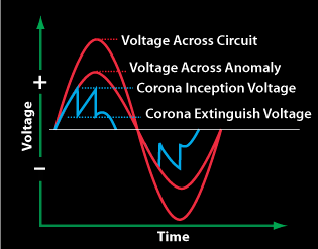
\includegraphics[width=\textwidth]{PartialDischarge}
    \caption{Partial Discharge}
    \label{fig:PartialDischarge}
\end{figure}

Partial discharge is a type of discharge in particular area occur because of transient in gas in oil insulation. Discharge occurs when current stress exceeds the defined critical value. The partial discharge level has a pronounced effect on the life of the current transformer\setlength{\parskip}{1em}.

As the current stress is increased, in the insulation system will result in Partial Discharge. As the current stress is reduced, Partial Discharge extinction will occur.
(MODIFIED)

The Partial Discharge cycle repeats rapidly during the peak values of a sine wave in current transformers. The excess energy dissipated during these repeating cycles causes deterioration of the insulation system resulting in premature failure of the Current Transformer.

Partial Discharge requires specialized equipment and cannot be characterized with standard dielectric testers. Partial Discharge can be minimized through the elimination of nano voids and contaminants during the design and manufacturing process. Construction materials and manufacturing process controls are designed for maximum product performance.

A BIL (Basic Insulation Level) rating on a Current transformer is an assurance that it will be able to routinely withstand power surges up to the given rating emanating from any number of common sources such as lightning, heavy motor start-ups, industrial load switching, grid overloads, \textit{etc}.

Recently, power grids, especially in metropolitan areas are reaching a level of saturation that results in a greater susceptibility to load variances, including lightning strikes. Consequently, AC switches and high voltage industrial equipment are exposed to voltage surges normally absorbed by the grid. BIL rated components are now being routinely specified for a much broader range of power control devices to greatly reduce the possibility of catastrophic system damage.

\begin{description}[style=nextline ]
 \item[Applied Voltage or Dielectric Test] A high voltage AC or DC test voltage is applied to the windings, and from the windings to ground. The test is designed to verify the adequacy of the system regarding coupling capacitance (AC) or resistance (DC).
 
 \item[Induced Voltage Test] The Induced Voltage Test reveals defects that might eventually result in a shorted turn and excessive excitation current. This test is important when winding layers are not properly insulated.
 
 \item[Partial Discharge (Corona) Test] The partial discharge test is a nondestructive method of identifying the potential for premature insulation breakdown. The test is capable of detecting small defects and nano voids in the insulation system that could lead to catastrophic transformer failure.
 \end{description}
 
Most of the research for Partial Discharge is done on medium voltage Current Transformers particularly on Cast epoxy resign. Need for analysis of High Voltage Current Transformers required to study effects of Partial discharge on performance. The insulation of CTs can be interested in the presence of common defects such as air bubbles or resin detachments at the interface between different parts of the component. The presence of such defects can be spotted during partial discharges tests \cite{sokolov1999effective}\setlength{\parskip}{0em}.
 
\subsection{On-line measuring system}

\subsubsection{On-Line partial discharge testing system for electrical systems}

There is \textbf{zero down time} associated with On-Line PD testing because the test is performed at normal operating voltage. Testing involves no external voltage or current sources\setlength{\parskip}{1em}.

Test equipment measures PD produced at voltages of 2400 volts and greater. The system is independent of load current. It is non-invasive testing that does not inject current into the system, nor does it subject the system to excessive voltage levels. Method is 100\% non-destructive and 100\% non-invasive systems.

The Online partial discharge testing gives warning of insulation failure so that maintenance plan can be done to avoid failure of instruments. Online testing gives the accurate condition of high voltage equipment including the effect of load, temperature and humidity. The on line testing are on destructive causing no interruption of service and performed under normal operating voltage, load and environmental conditions. No additional stress on the equipment under test no extra higher voltages stresses. In on line testing, the accuracy of PD measurement is more and more economical. The occurrence of PD can be located and can be repaired instantly.

The partial discharge activity will always lead to the dielectric breakdown of insulation inside the current transformer, The on line inspection techniques to measure partial discharge is developed by KEMA. A broad band high-frequency antenna is inserted inside to measure PD measurements during service. This technique is used for measuring PD in all HV equipment. The ultra high-frequency techniques are also used in many countries for on line detection. 

The diagnostic characteristics of current transformers and faulty insulation can be defined regarding partial activities and changes in capacitance and dielectric loss of defective area.

Contamination of defective area by dust particles, air bubbles in oil, the occurrence of small PD, destructive PD, progressive PD, will lead to the formation of gaseous. The gases thus formed will change the dielectric characteristics of insulation. The PD parameters can be concluded on Apparent charge magnitude, pulse repetition rate, discharge power, change in capacitance progressive PD.
 
The three methods for sensing PD used for on line measurements are acoustic, electromagnetic or frequency. In some cases, the combinations of these methods are 
also used as the diagnostic tool. The rough surface can be detected by using electromagnetic sensors, and the insulation strength can be detected by electric sensors and location of PD source by an acoustic sensor. The acoustic detection of partial discharge is an effective tool for the gaseous formed due to strong arcing in oil. The electric method can detect PD below 1000 pC, and acoustic method can detect above 10000 pC\setlength{\parskip}{0em}.

\subsubsection{Ultrasonic PD testing}
\setlength{\parskip}{0em}
Can pinpoint a suspected problem if the cable or accessory is not directly buried or is at least physically accessible.

The high-frequency ultrasonic components of PD are extremely short wave in nature, fairly directional and easy to isolate from background noise

The problem must be accessible.

\paragraph{Type of sensors advantages disadvantages\\}\setlength{\parskip}{1em}Electric direct connection to the test tap, or through high-frequency CT on the grounded wire, (\textquotedblleft Rogowski coils\textquotedblright) Additional sensors in bus duct, electrostatic shields, neural, \textit{etc}. High sensitivity Can be calibrated regarding apparent charge Approximate location of PD source All capabilities to trend data Use of PD pattern Recognition technology Sensors configuration can match for better noise rejection De-energizing for sensors installation.

Electromagnetic antenna easy to use possible assessing external PD problems including PD in the bushings Serving as noise (corona) channel High disturbances Only discharges of extremely high level can be detected Difficult to distinguish an equipment having problems from surrounding equipment.

Acoustic Piezo-accelerometer placed on transformer tank Easy to install Capability detecting acoustic emission magnitude and trend, Pulse repetition rate and trend Localizing a source of PD using signal time of arrival to different locations Low sensitivity Minimal detecting apparent charge \textgreater 10,000 pC Responded to rain, sleet, electrical disturbances in the station The level of signal depends on coupling between the sensor and surface Effect of design (variables inside the tank) on the propagation of sound wave.

The portable universal PD analyzer is used for different applications to detect PD in high voltage instruments transformers. The PD analyzer monitors waveforms for different power frequency simultaneously using many sensors and identifies PD pulses. The radio frequency pulses will identify the capacitance difference. The frequency band, 1 MHz to 20 MHz, can be selected by the sensors to detect PD in instruments. Electronic processing of signals, phase and frequency selection, time delay and signal comparison are done with the sensors simultaneously.

The modern techniques of on line measurement of PD gives a high sensitivity of PD measurement as comp aired to testing in the laboratory. The on line testing used as a diagnostic instrument. The on line testing can distinguish between small discharge and destructive discharge which affect electrical equipment to the critical status\setlength{\parskip}{0em}.

\subsection{Off line measuring system}

\subsubsection{Off-line testing techniques}
\begin{itemize}
\item Power Factor/Dissipation Factor Testing
\item Very Low-Frequency Testing (VLF)
\end{itemize}

\subsubsection{In-service testing techniques}
\begin{description}[style=nextline]
\item[Power Factor/Dissipation Factor Testing] This measurement is effective in identifying weak insulation and knowing reasons of potential hazards before the occurrence of a failure. Test process has no overstressed effect on insulation and gives the information of insulation strength of instrument.

\item[Very Low Frequency (VLF) Testing] This measurement process damages the insulation during the test. The supply with low frequency is applied to insulation. This process has the capability of locating potential failure at sites. VLF has the advantage of portability with low energy requirements, which results in much smaller test sets. Voltage is raised to above the Partial Discharge inception voltage which helps in creating partial discharge to occur.
\end{description}

\section[Effect of Partial Discharge on Electrical Equipments]{Effect of Partial Discharge on\\Electrical Equipments}
\subsubsection{Effect of partial discharge}
\begin{enumerate}
\item Partial discharge in Current transformers reduces dielectric strength of solid insulating resulting in the early break down of the instrument.

\item The partial discharge process can cause contamination of oil resulting in a change of insulating properties which will result in the early breakdown of the system.

\item Partial discharge measurement provides information on the aging effect on insulation which can help in deciding the life of the instrument.

\item Partial ~discharge ~identification ~indicates ~type ~of ~fault. The ~digital measurement system gives the inside information about discharge, the effect of environmental interference and strong information about maintenance required and quality of insulation. 
\end{enumerate}


\section{Predictions from Partial  discharge }
The partial discharge characteristics are different for different void conditions. The electrical trees formed depend on charge value and dimensions of voids. The amplitude of pulse, shape of the pulse width, rise and fall time depends upon the applied voltage and insulation strength. Discharge occurs in every half cycle due to the disturbances of voids\setlength{\parskip}{1em}.


Predictions of failure can be done from Electrical trees formed due to discharge in insulation. The penetration of tree in insulation, its branches, size, the formation of a void, dimensions of voids will help in assessing breakdown and collapse of an electrical instrument. 

Manufacturing process or insulation deterioration due to normal service operating conditions.

Partial discharge testing is a preventive detection tool which can alarm the potential failures due to insulation level of electrical equipment.

The Partial Discharge helps to identify discharge in insulation of cables, splices, transformers. The partial discharge testing is nondestructive testing\setlength{\parskip}{0em}.

\section{Study of Various Instruments Which Detects Partial Discharge in  High Voltage Instrument}

\subsection{Expert partial discharge analyzer with reflectometer - R2100}
R2100 shown as a complete kit with a variety of Partial Discharge Sensors
\begin{itemize}
\item Most Advanced PD Analyzer in the World
\item 12 PD Channels 
\item Noise Cancellation 
\begin{itemize}
\item Pulse Shape 
\item Pulse Polarity 
\item Pulse Comparison 
\item Time of Arrival 
\item Specialized software filters
\end{itemize}
\item TDR capability to assist in determining location of defect 
\end{itemize}

\begin{figure}[h!]
    \centering
    \begin{subfigure}[b]{0.32\textwidth}
        \centering
        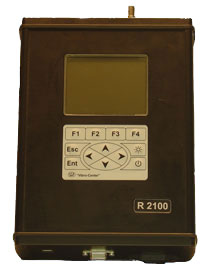
\includegraphics{251}
    \end{subfigure}
    \\
    \begin{subfigure}[b]{0.32\textwidth}
        \centering
        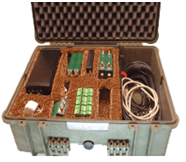
\includegraphics{252}
    \end{subfigure}
    \hspace{1cm}
    \begin{subfigure}[b]{0.32\textwidth}
        \centering
        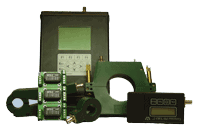
\includegraphics[height=4cm]{253}
    \end{subfigure}
    
    \caption{Expert Partial Discharge Analyzer with Reflectometer }
    \label{fig:Expert Partial Discharge Analyzer with Reflectometer }
\end{figure}

The instrument can measure external temperature, humidity. It has total 12 channels with the help of sensors. All PD channels have identical isolated input circuitry with protection and high pass filters. The frequency band is 0.5 to 10 MHz. This instrument eliminates the noise generated due to high voltage instrument in the substation. The instruments are fitted with noise filters. Almost all technologies that may found combined in different instruments on the market. PD channels may be flexibly configured to use one or another noise filtering technology or a combination of technologies \setlength{\parskip}{1em} \cite{gurin1975measurements}.

This instrument is an analyzer with the principle of the reflectometer. Reflectometer will help in identifying the defective location. This helps in identifying faults in long distance cables. The instrument is capable of recording up to three-time domain reflectograms per channel with different trigger levels. The trigger level may be automatically adjusted to signal level or pre-determined by the operator.

Partial data can be stored in this instrument. The instrument has 48 phase windows and 32 magnitude windows with a single dynamic range of 70 dB without gain adjustment. A full suite of software included that allows the user to download all data to a PC, perform analysis and present the data\setlength{\parskip}{0em}.

\subsection{Partial discharge analysis system}
 This instrument is an advanced system for analysis of partial discharge.
 
\begin{figure}[h!]
    \centering
    \begin{subfigure}[b]{0.30\textwidth}
        \centering
        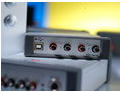
\includegraphics[height=3.5cm]{254}
    \end{subfigure}
    \begin{subfigure}[b]{0.60\textwidth}
        \centering
        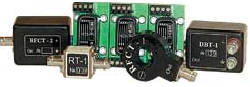
\includegraphics[height=3cm]{255}
    \end{subfigure}
    
    \caption{Partial Discharge Analysis System}
    \label{fig:Partial Discharge Analysis System}
\end{figure}

This instrument measures in high precision for high voltage equipment for insulation strength.Using galvanic isolation, it can minimize noise and most safe for measuring cable insulation for the distance of 2 kM. The instrument is light in weight and easy for portability\setlength{\parskip}{1em}. 

 
These are Vibro center equipment with Partial discharge sensors fitted inside. 

Sensors measure and diagnose partial discharge pulse. The sensors are perfect in the precision of measurement. Reliability of these instruments is very high. Sensors capture partial discharge pulses and give signal to the control unit. This instrument is designed for a load capacity of 50 $\Omega$ and can be attached directly to the measuring instruments\setlength{\parskip}{0em}.
 
\subsection{DB series sensors}
The DB series is used for high voltage equipment, bushings, current transformers. These sensors control dissipation factor and current and sense partial discharge phenomenon inside the current transformer and bushing. The insulation conditions inside the transformers are signaled with the sensors. The over voltage protection sensors are also fitted inside the instruments. These sensors are covered in the protective shield to avoid physical damage. The bushing of transformers is covered for protection as the high voltage equipment can undergo switching impulse and lightning threat. The switching impulse is not more than 1.3 kA for an instrument of 145 kV. The overvoltage protection is also sensed in the DB series. Various types of sensors depending on fitment requirement on instrument and bushing can be made suitable. These sensors are connected to PD measurement instrument.

The DB series sensors are designed based on the application are classified as:
\begin{itemize}
\item Operating voltage of bushing from 72 kV to 400 kV
\item As per the fitment on Equipment dimensions of sensors decided for ease fitment
\end{itemize}

\subsubsection{Sensor DB-1}
\begin{figure}[h!]
    \centering
    \begin{subfigure}[b]{0.49\textwidth}
        \centering
        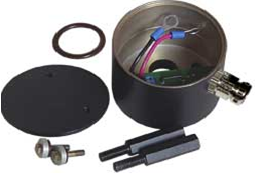
\includegraphics{256}
    \end{subfigure}
    \begin{subfigure}[b]{0.49\textwidth}
        \centering
        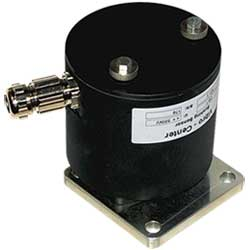
\includegraphics[height=4cm]{257}
    \end{subfigure}
    
    \vspace{3em}
    
    \begin{subfigure}[b]{0.49\textwidth}
        \centering
        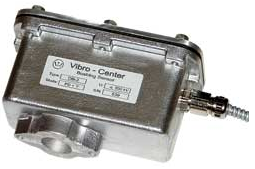
\includegraphics{258}
    \end{subfigure}
    \begin{subfigure}[b]{0.49\textwidth}
        \centering
        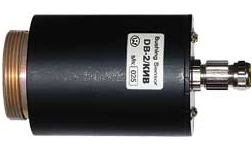
\includegraphics[height=4cm]{259}
    \end{subfigure}
    
    \caption{Sensor DB-1}
    \label{fig:Sensor DB-1}
\end{figure}

Sensor DB-1 are suitable for oil filled bushing transformers. These sensors are easy to mount on bushings of transformers for voltage above 132 kV. With mechanical fitting with the seal and study on bushings. The mechanical flange is provided for fitment on the bushing.

\subsubsection{DB-1 sensor structural variation}
These sensors are suitable for 110 kV operating voltage and easy for fitment on bushing fitted on transformer top cover.

These sensors are fitted in the metallic case and have protection for a high current pulse. The operating voltage above 66 kV \cite{gurin1993field}.

\subsubsection{Sensors for bushings of transformers}
The transformer bushing is filled with the oil and requires current monitoring sensors. These sensors have current measuring system and fitting arrangement on the body of transformers.

\begin{figure}[h!]
    \centering
    \begin{subfigure}[b]{0.49\textwidth}
        \centering
        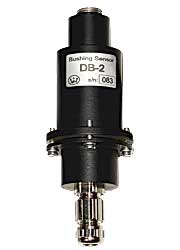
\includegraphics{2510}
    \end{subfigure}
    \begin{subfigure}[b]{0.49\textwidth}
        \centering
        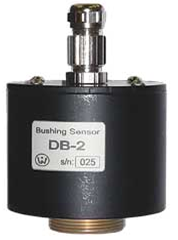
\includegraphics{2511}
    \end{subfigure}
    
    \caption{Sensors for bushings of transformers}
    \label{fig:Sensors for bushings of transformers}
\end{figure}

For the sensors which are produced by \textquotedblleft Trench,\textquotedblright \textquotedblleft GE\textquotedblright with the operating voltage of 300 kV and more it is these are possible to use the sensor that is shown in the picture. This sensor has a pilot thread of Ì 30 * 1,5 mm.

Three more sensor's varieties, which are produced by our firm, have a less spread, so they are not shown here. They have other types of mounting thread and the use of spring movable sensor contacts with the bushing test tap.

\subsubsection{Sensors DB-TT}
\begin{figure}[h!]
\centering
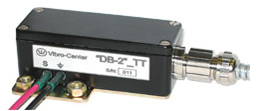
\includegraphics{2512}
\caption{Sensors DB-TT}
\label{fig:Sensors DB-TT}
\end{figure}

Sensors ~DB-2/TT ~these are ~used to ~know ~the insulation strength ~of ~current transformer. These sensors are fitted inside the terminal box.

\subsection{RFCT sensors}
These sensors are high-frequency transformers of current. Compared with usual transformer they separate in a current, which runs in the conductor, high-frequency impulses in the range from 0,5 MHz to 50 MHz from partial discharge. These sensors don’t record the current rippling of commercial frequency\setlength{\parskip}{1em}.

These are fitted on the grounding conductor, transformer neutral, and ground of the transformer tank, braiding ground of power cable, coupling capacitor ground and in the compensating circuit. 

The choice of the sensor mounting place depends on the controlled equipment type and task. For the task solution exact method of partial discharge recording is created. So the RFCT sensors embodiment is different, subject to the type of the seat for the sensor.

The special protective insulation, which is meant for protection of device measuring chain from external voltage, is not provided in the sensor’s construction. Therefore RFCT sensors could be mounted on the piece of equipment, which is the ground element or which is reliably attached to the ground only. In another case, it is necessary to envisage the use of additional insulation between the sensor case and the conductor line, in which the existence of partial discharge impulses is assumed\setlength{\parskip}{0em}. 

\begin{figure}[b!]
    \centering
    \begin{subfigure}[b]{0.49\textwidth}
        \centering
        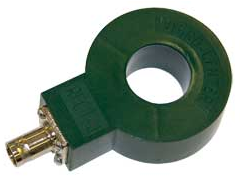
\includegraphics[width=\textwidth, height=6cm,keepaspectratio]{2513}
        \caption{RFCT-1 sensors }
    \end{subfigure}
    \begin{subfigure}[b]{0.49\textwidth}
        \centering
        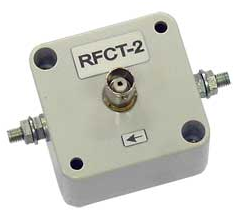
\includegraphics[width=\textwidth, height=6cm,keepaspectratio]{2514}
        \caption{RFCT-2 sensors }
    \end{subfigure}
    
    \begin{subfigure}[b]{0.49\textwidth}
        \centering
        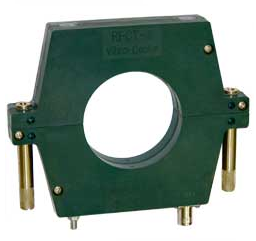
\includegraphics[width=\textwidth, height=6cm,keepaspectratio]{2515}
        \caption{RFCT-4 sensors }
    \end{subfigure}
    \begin{subfigure}[b]{0.49\textwidth}
        \centering
        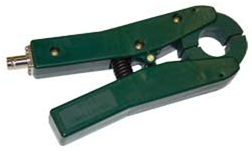
\includegraphics[width=\textwidth, height=6cm,keepaspectratio]{2516}
        \caption{RFCT-5 sensors }
    \end{subfigure}
    
    \begin{subfigure}[b]{0.49\textwidth}
        \centering
        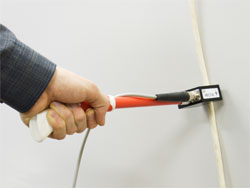
\includegraphics[width=\textwidth, height=6cm,keepaspectratio]{2517}
        \caption{RFCT-5 sensors }
    \end{subfigure}
    \begin{subfigure}[b]{0.49\textwidth}
        \centering
        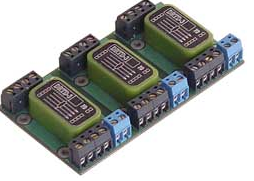
\includegraphics[width=\textwidth, height=6cm,keepaspectratio]{2518}
        \caption{RFCT-6 sensors }
    \end{subfigure}
    
    \caption{Types of RFCT Sensors to Detect Partial Discharge}
    \label{fig:Types of RFCT Sensors to Detect Partial Discharge}
\end{figure}

\subsubsection{RFCT-1 sensors}
The inside sensor core is implemented in the form of a hoop. The close gaps are necessary for sensitivity increasing of the measuring circuit. It can be explained by the range of the registered frequency. When mounting the sensor, it is necessary to break the metering circuit and to let the conductor through the sensor. The RFCT-1 sensor is connected with the device due to standard coaxial cable and BNC socket. Inside diameter of the sensor is 22 mm. 

\subsubsection{RFCT-2 sensors}
Constructively the sensor has a series of blocking capacitor of 6800 pF and pulse transformer inside. So RFCT-2 sensors are aimed at impulses registration of partial discharges in the high-voltage circuit breaker, the cell of the switchgear and control gear and in the cable lines, which are connected with it. Also, these sensors are used for impulses registration of partial discharges in other high-voltage equipment, where other RFCT sensors constructively cannot be used.

Electrically, the sensor does not let through power current through. It lets through partial discharge impulse only.

\subsubsection{RFCT-4 sensors}
The RFCT-4 sensor has the biggest inside diameter. These sensors are aimed at the installation on the transformer neutral and equipment ground bus. The sensor has a split case. It consists of 2 parts for the ease of installation on the bus, which has a rigid attachment. The sensor’s inside diameter is 68 mm.

Inside the sensor, there is a protective screen that may be connected to the ground through the ground bolt. This enables to improve the safety of measuring implementation.

\subsubsection{RFCT-5 sensors}
Constructively it is produced in the form of the current clamp and is aimed at the on-line control of the equipment insulation condition.

Sensors of this type are available with the device R-400. Originally this sensor is developed for the partial discharges measuring. However it can be used as the usual RFCT type sensor. 
 
The sensor is inside diameter, by which wire passes, is 24 mm.

\subsubsection{RFCT-6 sensors}
RFCT-6 sensors are aimed at online monitoring of electrical equipment (cable, cable box, \textit{etc}.) to identify partial discharges presence in equipment.

The RFCT-6 sensor is a partial discharges indicator only. Its data cannot be used for the appraisal of defect degree.

The sensor is connected to the device. The sensor is brought reasonably close to the conductor, in which the partial discharge detection is planned. The current direction in the wire must coincide with sensor pointer or be opposite. If turn the sensor at an angle of 90 degrees, then you cannot register the partial discharge.
 
The closer the sensor approach to conductor is the more amplitude on its output.

\subsection{DRTD-3 sensor}
A DRTD-3 sensor is aimed at the partial discharge recording in the stator winding of electric machine. As an antenna thermostats, which are put into electrical machine winding on the producer factory, are used. The sensor is included in the temperature measurement circuit break. The high-frequency component is single out from the complete signal from thermostats due to the sensor. High-frequency component carries the information about partial discharge in the winding. Sensor’s construction was designed in a way, that its involvement in the measurement circuit will not lead to significant accuracy in the process of the temperature measurement.

\subsection{KS-60 sensors}
\begin{figure}[h!]
\centering
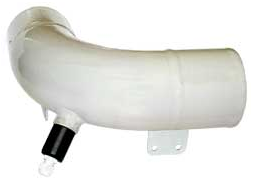
\includegraphics{2519}
\caption{KS-60 sensors}
\label{fig:KS-60 sensors}
\end{figure}

KS-60 ~sensor is created ~especially for the ~practical ~realization of the ~partial discharges method of recording in Transformers, or rather for the corona impulse tune-out. These impulses are a undesired signal. They are like a partial discharge impulse. Usually, it has a high amplitude and leads to the authenticity of monitoring system work of partial discharges in Transformers, and repeatable measurements by portable devices are inadmissibly low. So, despite these sensors, bulkiness, and difficulties with installation, the partial discharge monitoring system operation without using of KS-60 corona sensors (or such-like ) is impossible in the transformer.\\
 
As for physical aspect, the sensor of corona discharge impulses is aimed at the recording of the magnetic field tangential component, which appears the the transformer ~bushing ~bar ~while the high-frequency impulse ~flows ~through ~it. Depending on the direction of one impulse flow, inside or outside of transformer, signal polarity is changed on the sensor output.

\subsection{AR-1 sensor}
\begin{figure}[h!]
\centering
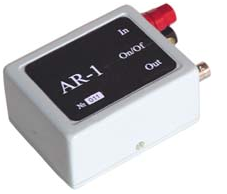
\includegraphics{2520}
\caption{AR-1 sensor}
\label{fig:AR-1 sensor}
\end{figure}

This sensor is aimed at the reference forming, which is necessary to partial discharge binding. The AR-1 sensors input signals could have different amplitude range, all the way from tens millivolts to supply voltage of 220 V. Rectangular impulse is formed in the sensor output. It has an even period as a input single. Input circuit and output circuit has a galvanic isolation for the voltage to 1500 V. Galvanic isolation allows excluding circuit interference between themselves and between the controlled object and measuring device. It is very important when the reference voltage for the phase binding is taken from another object made under high-voltage substation. Too small sensor input current, which numerically is equal to parts of microampere, extends the range of the sensor use. For example, when measuring on the transformer bushings, the sensor could be connected parallel to DBT-1 sensor, without error injection in the partial discharge measurements. The sensor could be used as an external synchronization of R400 device. The sensor has an inside power supply from two AA batteries. One complete set of batteries works for about 10 hours. The sensor is turned on and turned off by the power switch.

\subsection{RT-1 isolating transformer}
\begin{figure}[h!]
\centering
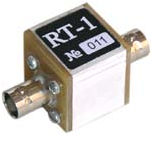
\includegraphics[scale=1.5]{2521}
\caption{RT-1 isolating transformer}
\label{fig:RT-1 isolating transformerr}
\end{figure}

This sensor is a high-frequency isolating transformer. The sensor is used in the partial discharge measuring circuit, where it may be circulating currents flow in the measuring and grounded circuits or between the measuring line. RT-1 sensor separates the high-frequency signal component of partial discharge from the signals of commercial frequency. The epoxy-filled isolating transformer is in the isolated case. It has a high-frequency transformation coefficient, which is equal to one.

\subsection{GKI-2 calibration oscillator}
\begin{figure}[h!]
\centering
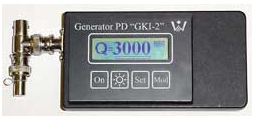
\includegraphics[scale=1.5]{2522}
\caption{GKI-2 calibration oscillator}
\label{fig:GKI-2 calibration oscillator}
\end{figure}

Small ~calibration ~oscillator ~GKI-2 ~is used for ~calibration of ~partial ~discharge registration circuit. Device injects electric charge into the controlled object and metering circuits. This makes it possible to calibrate a metering circuits given attenuation in the device before measuring. The injected charge circuit is connected through BNC connector on the left part of the device case.\\

The device injects a charge of 3nC into controlled object and metering circuit. The repetition frequency is 25 kHz. The leading edge of a pulse is about 5 ns. Calibration is in the sensitivity test of the measuring system. Sensitivity is set in nC/V. For example, the device registered the charge for 3nC, which is injected by the generator with an amplitude of 500 mV. Consequently the sensor's sensitivity is 3nC / 0.5V = 6nC/V.

\subsection{Ultrasonic and acoustic emission}
All operating equipment produces a broad range of sound. The high-frequency ultrasonic components of these sounds are an extremely short wave in nature, and a short wave signal tends to be fairly directional. It is therefore relatively straightforward to isolate these signals from background noises and detect their exact location. Also, as subtle changes begin to occur in electrical and mechanical equipment, the nature of ultrasound allows these potential warning signals to be detected early, before actual failure\setlength{\parskip}{1em}.

Airborne ~~ultrasound ~instruments, ~~often ~referred ~to ~as ~\textquotedblleft ~ultrasonic ~translators,\textquotedblright\\provide information two ways: qualitatively, due to the ability to \textquotedblleft hear' ultrasounds through a noise isolating headphone, and quantitatively, via incremental readings on a meter. This is accomplished in most ultrasonic translators by \textcopyright~2004 SKF Reliability Systems All Rights Reserved 2 MB04025 - Partial Discharge Analysis High voltage applications include insulators, cable, switchgear, buss bars, relays, contactors, and junction boxes. In substations, components such as insulators, transformers and bushings may be tested.

The method for detecting electric arc and corona leakage is similar to the procedure used to detect acoustic emissions from mechanical sources. Instead of listening for a rushing or rubbing sound, a user listens for a crackling or buzzing sound. In some instances, as in trying to locate the source of radio/TV interference or in substations, the general area of disturbance may be located with a gross detector such as a transistor radio or a wide-band interference locator. Once the general area has been located, the scanning module is utilized with a general scan of the area. The sensitivity is reduced if the signal is a too strong .electronic process called \textquotedblleft heterodyning,\textquotedblright which accurately converts the ultrasounds sensed by the instrument into the audible range where users can hear and recognize them through headphones \cite{sokolov1995experience}.

Although the ability to gauge intensity and view sonic patterns is important, it is equally important to be able to \textquotedblleft hear\textquotedblright the ultrasounds produced by the various equipment. That is precisely what makes these instruments so useful; they allow analysts to confirm a diagnosis on the spot by being able to discriminate among various equipment sounds.

The reason users can accurately pinpoint the location of a particular ultrasonic signal in a machine is due to its high frequency / short wavelength. Most of the sounds sensed by humans range between 20 Hz and 20 kHz (20 cycles per second to 20,000 cycles per second). They tend to be relatively gross when compared with the sound waves sensed by ultrasonic translators. Low-frequency sounds in the audible range are approximately 1.9 cm. to 17 meters in length, whereas ultrasounds sensed by ultrasonic translators are only 0.3 - 1.6 cm long. Since ultrasound wavelengths are magnitudes smaller, the ultrasonic environment is much more conducive to locating and isolating the source of problems in loud plant environments\setlength{\parskip}{0em}.

\subsubsection{Using ultrasonic and acoustic emission for partial discharge}
Ultrasonic testing is often used for evaluation at voltages exceeding 1,000 volts, especially in enclosed switchgear. This is especially useful in identifying tracking problems. In enclosed switchgear, the frequency of tracking greatly exceeds the frequency of serious faults, which can be identified using techniques such as infrared thermography\setlength{\parskip}{1em}.

When electricity escapes in high voltage lines or when it jumps across a gap in an electrical connection, it disturbs the air molecules around it and generates ultrasound. Often this sound will be perceived as a crackling or frying sound; in other situations, it will be heard as a buzzing sound.

There are three basic electrical problems that can be detected using ultrasound\setlength{\parskip}{0em}: 
\begin{description}
\item[Corona:] When the voltage on an electrical conductor, such as an antenna or high voltage transmission line exceeds the threshold value, the air around it begins to ionize to form a blue or purple glow.

\item[Tracking:] Often referred to as \textquotedblleft baby arcing,\textquotedblright follows the path of damaged insulation.

\item[Arcing:] An arc occurs when electricity flows through space. Lightning is a good example. 
\end{description}

The process can be used to detect both end winding (Phase to Phase) and slot section (Phase to Earth) discharge.

\subsubsection{Partial discharge pattern recognition of current transformers using an ENN  extension neutral network}
Extension-neural-network (ENN)-based recognition method to identify the partial-discharge (PD) patterns of high-voltage current transformers (HVCTs). First, a commercial PD detector is used to measure the three-dimensional (3D) PD patterns of HVCTs, then three data preprocessing schemes that extract relevant features from the raw 3-D PD patterns are presented for the proposed ENN-based classifier. Than traditional neural networks. The ENN has the advantages of high accuracy and noise tolerance, which are useful in recognizing the PD patterns of electrical apparatus. 

\subsubsection{Partial discharge sensors and bushing conduction current sensors, that are being produced by Vibro-Center}
Primary sensors are the base of all measuring diagnostic system. Functionality and operating efficiency of all measuring systems depend on sensors precision and reliability.

Vibro-Center produces a wide variety of sensors for the control operation of the equipment, which registers partial discharges. All these sensors are meant for registration of \textquotedblleft electric\textquotedblright partial discharges in high-voltage power equipment. All these sensors are aimed at working with a standard load of 50 $\Omega$, so they can be used for working with measuring devices that are produced by other companies. A current transformer is very important apparatus in electrical power system the measurement and protection. Partial discharges in a current transformer are often a predecessor of a serious fault. For this reason, partial discharge measurements are nondestructive diagnostic tool to monitor the insulation condition of a current transformer. The simple Partial Discharges (PD) detection is not enough to decide against intervening, so the localization is necessary to assess the risk and to plan corrective actions.

\pagebreak 
\section{Research Gap}
Various literature is available on partial discharge phenomenon, causes, measurement, and testing of electrical equipment. But very few data available on high voltage oil filled current transformers 145 kV, where the primary current is very high from 100 Amp to 3000 Amp\setlength{\parskip}{1em}.
 
The effect on Insulation medium used has high electrical stress due to high current capacity. The failure of current transformers in the system will lead to the breakdown of the complete system. Hence need for analysis is required to study the effect of Partial Discharge on High Voltage Current Transformers 145 kV up to 3000 Amp.

There is need to develop and study some models in Simulink to verify and analysis Partial discharge pulses. As Partial Discharge phenomenon starts because of contamination in insulating material or presence of a void in insulating material, due to both insulation strength gets weakens and discharge of charge starts at weak points. Hence it is necessary to study the effect various voids on the performance of current transformers during steady state conditions and short circuit and transient conditions. The presence of voids in the insulating material represents capacitance which causes discharge phenomenon in the insulating material. The study is required for different waveforms for different void conditions, nature of pulses, amplitude, wavelength from the Simulink model during steady state and short circuit and transient conditions. Need to study the difference in ratio error, phase error for accuracy test during steady state and transient conditions.

Thus need for study effect of voids on partial discharges, the study of mathematical model and effect of steady state conditions and short circuit and transients conditions and analysis of waveforms to make improvements in servicing, manufacturing and designing of high voltage oil filled current transformers for un-interruption in power supply.
\setlength{\parskip}{0em}